\documentclass[12pt]{article}

\usepackage{amsmath}
\usepackage{graphicx}
\graphicspath{ {./images/} }
\usepackage[utf8]{inputenc}
\usepackage[russian]{babel}
\usepackage{geometry}
 \geometry{
 a4paper,
 left=20mm,
 right=20mm,
 top=20mm,
 bot=20mm,
 }

\begin{document}

\begin{titlepage}
\begin{center}
    {\small НАЦИОНАЛЬНЫЙ ИССЛЕДОВАТЕЛЬСКИЙ УНИВЕРСИТЕТ ИТМО} \\
    {\small Факультет систем управления и робототехники} \\
    \vspace*{10\baselineskip}
    {\LARGEМоделирование динамических систем} \\
    \ \\
    {\LARGEЛабораторная работа №2} \\
    \ \\
    {\LARGEУстойчивость нелинейных систем} \\
    \ \\
    Вариант 2 \\
    \vspace*{10\baselineskip}
    \hfill {\small Выполнил студент:} \\
    \hfill {\small Кирбаба Д.Д. R3338} \\
    \ \\
    \hfill {\small Преподаватель:} \\
    \hfill {\small Семенов Д.М.} \\
    \mbox{}
    \vfill {\smallг. Санкт-Петербург\\2023}
\end{center}
\end{titlepage}

\section*{Задание 1}
Дана следующая нелинейная система:
\[
\begin{cases}
    \dot{x} = -3x + y\\
    \dot{y} = -x - 2y - \frac{y}{|y| + 1}
\end{cases}
\]\\
Необходимо найти все точки равновесия системы, линеаризовать систему около точек равновесия и исследовать устойчивость линеаризованной системы, построить функцию Ляпунова и доказать глобальную устойчивость нелинейной системы, отобразить графики линейной (линеаризованной) и нелинейной систем.\\
\ \\
Для поиска точек равновесия системы, необходимо приравнять левую часть (производные) к нулю и решить систему:
\[
\begin{cases}
    -3x + y = 0\\
    -x - 2y - \frac{y}{|y| + 1} = 0
\end{cases}
\Rightarrow
\begin{cases}
    x = \frac{y}{3}\\
    -\frac{y}{3} - 2y - \frac{y}{|y| + 1} = 0
\end{cases}
\Rightarrow
\begin{cases}
    x = 0\\
    y = 0
\end{cases}
\]\\
Итого, имеет единственную точку равновесия $(x=0,\ y=0)$.\\
\ \\
Линеаризуем нашу систему около положения равновесия, то есть сконструируем систему $\dot{\Delta} = A\Delta$, где $\Delta = x - a = x$. В данной записи $x$ - двумерный вектор состояний системы, а $A$ - матрица частных производных.\\
\ \\
Составим матрицу Якоби системы:
\[
    A = \begin{bmatrix}
\frac{\delta f_1(x,\ y)}{\delta x} & \frac{\delta f_1(x,\ y)}{\delta y}\\
\frac{\delta f_2(x,\ y)}{\delta x} & \frac{\delta f_2(x,\ y)}{\delta y}
\end{bmatrix}_{x=a} = 
\begin{bmatrix}
-3 & 1\\
-1 & -3
\end{bmatrix}
\]
Теперь исследуем линеаризованную систему на устойчивость (анализом собственных чисел матрицы $A$):
\[
\lambda_1 = -3 - i, \ \lambda_2 = -3 + i
\]
Так как значение $\max{Re(\lambda(A))} = -3 < 0$, то по соответствующей теореме положения равновесия $(x=0, \ y=0)$ локально асимптотически устойчиво. Положение равновесия в данном случае имеет вид устойчивого фокуса. А это значит, что и исходная нелинейная система локально устойчива в данном положении.\\
\ \\
Докажем глобальную устойчивость нелинейной системы, для этого сформируем функцию Ляпунова:
\[
V(x, \ y) = x^2 + y^2, \ V(x, \ y) > 0, \ V(0, \ 0) = 0
\]
\[
\begin{split}
    \dot{V}(x, \ y) = 2x\dot{x} + 2y\dot{y} = 2x(-3x + y) + 2y(-x - 2y - \frac{y}{|y| + 1}) \\
    = -6x^2 - 4y^2 - \frac{2y^2}{|y|+1} < 0, \ \forall (x, \ y) \in R^2 \setminus \{0\}
\end{split}
\]
Исходя из этих вычислений, следует, что для введенной функции Ляпунова $V(x, \ y)$ и исследуемой нелинейной системы выполняются условия теоремы об асимптотической устойчивости, а значит, нулевое решение системы глобально
асимптотически устойчиво.\\
\ \\
Предоставим графики компонент состояния линеаризованной и нелинейной систем:\\

\begin{figure}[h!]
    \centering
    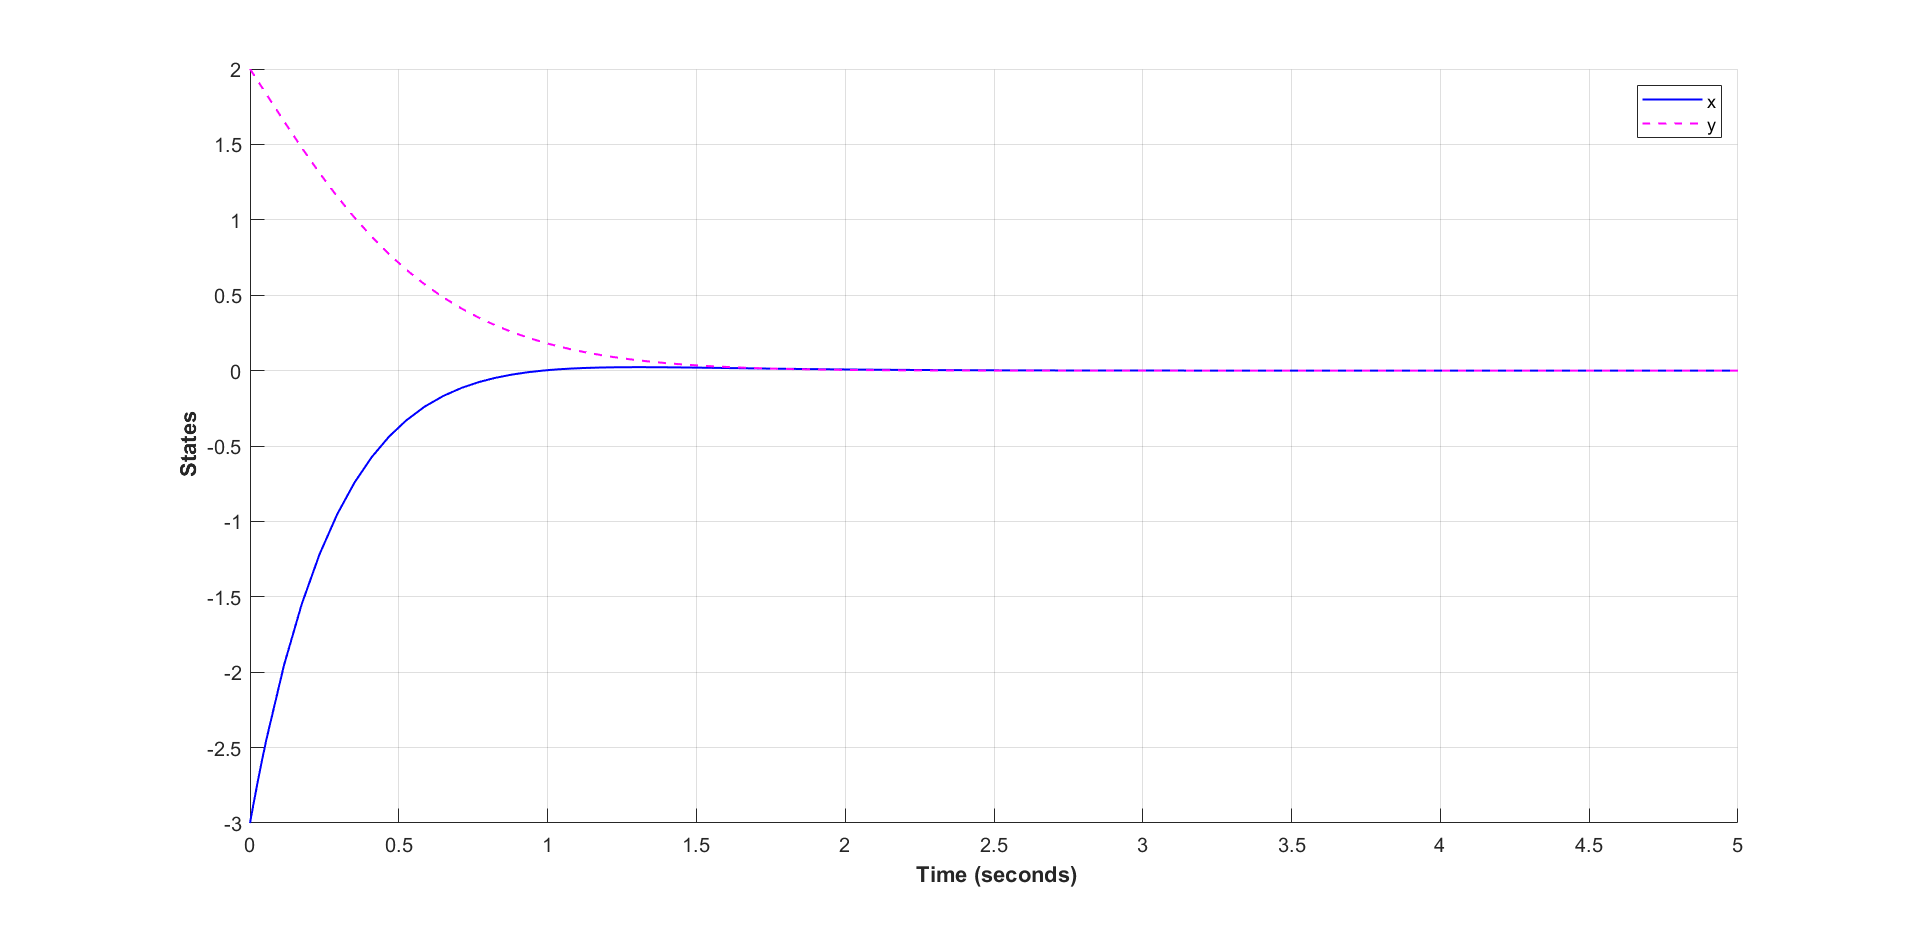
\includegraphics[width=\textwidth]{lin_states}
    \caption{компоненты вектора состояний линеаризованной системы}
    \label{fig:lin_states}
\end{figure}

\begin{figure}[h!]
    \centering
    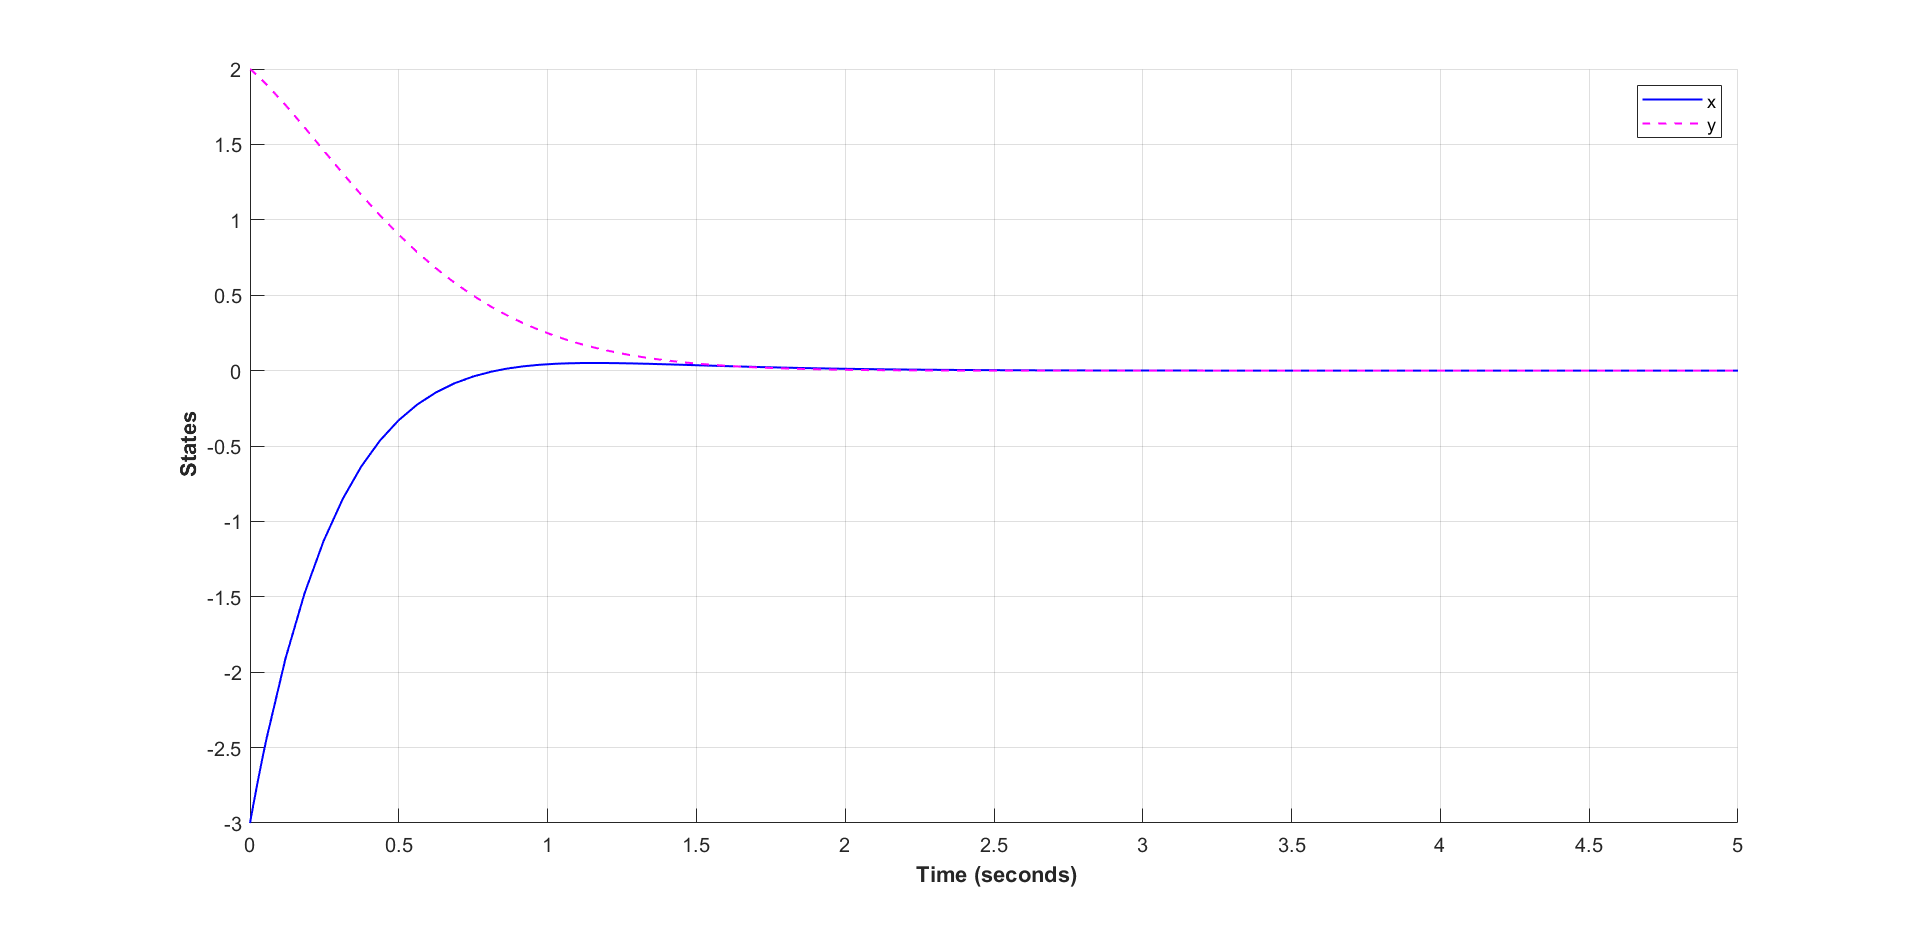
\includegraphics[width=\textwidth]{non_lin_states}
    \caption{компоненты вектора состояний исходной нелинейной системы}
    \label{fig:non_lin_states}
\end{figure} \\
Как видно, обе системы устойчивы, что подтверждает вычисления и анализ, проведенный выше.

\section*{Задание 2}
Дана следующая нелинейная система:
\[
\begin{cases}
    \dot{x} = Ax + b\xi, \ \sigma=c^Tx,\\
    \xi = \varphi(\sigma, t),
\end{cases}
\]\\ где
\[
A = \begin{bmatrix}
-1 & 1\\
-2 & -3
\end{bmatrix}, \ b = \begin{bmatrix}
0\\
1
\end{bmatrix}, \ c = \begin{bmatrix}
1\\
0
\end{bmatrix}, \ \xi = \sin{(\sigma)}
\]\\
Необходимо доказать экспоненциальную устойчивость системы, используя круговой критерий.
\subsubsection*{"Секторное условие"}
\[
\mu_1 \leq \frac{\sin{\sigma}}{\sigma} \leq \mu_2, \ \sigma \neq 0, \ \forall t \in (0, \infty)
\]
\[
\mu_1 \sigma \leq \sin{\sigma} \leq \mu_2 \sigma \Rightarrow_{derivative}\Rightarrow \mu_1 \leq \cos{\sigma} \leq \mu_2
\]
\[
\mu_1 = -1, \ \mu_2 = 1
\]
\begin{figure}[h]
    \centering
    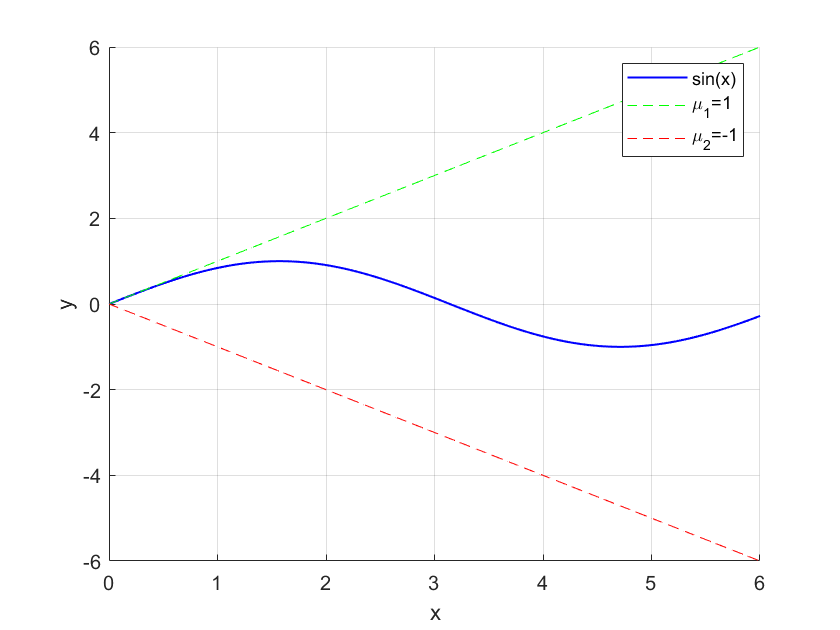
\includegraphics[width=0.7\textwidth]{sector_criterion_2}
    \caption{круговой критерий}
    \label{fig:sector_criterion_2}
\end{figure} \\
Из рисунка выше следует, что "секторное условие" выполнено.
\subsubsection*{Проверка мнимых собственных значений}
Вычислим собственные значения матрицы $A$:
\[
\lambda_1 = -2 - i, \ \lambda_2 = -2 + i
\]
Матрица $A$ не имеет чисто мнимых собственных значений $\Rightarrow$ условие выполнено.
\subsubsection*{Асимптотическая устойчивость линейной системы}
Асимптотическая устойчивость системы при $\xi = \mu_0 \sigma$.
Поскольку значение $\mu_0$ выбирается из интервала $[\mu_1, \mu_2]$, то можно
выбрать $\mu_0=0$. Тогда исследуемая система будет иметь вид $\dot{x} = Ax$. Поскольку собственные числа матрицы $A$ уже известны и они имеют отрицательную вещественную часть, то $\Rightarrow$ линейная система асимптотически устойчива, а значит, условие выполнено.
\subsubsection*{"Частотное условие"}
Вычислим передаточную функцию системы:
\[
W(\lambda) = c^T(A-\lambda I)^{-1}b = -\frac{1}{\lambda^2 + 4 \lambda + 5}
\]
Возьмем $\lambda = i \omega$ и проверим следующее неравенство:
\[
Re\{[1 + \mu_1 W(i \omega)][1 + \mu_2 W(i \omega)]^*\} > 0, \ \omega \in [-\infty, \ +\infty]
\]
Так как $\mu_1 = 0 и \mu_2 = 1$, то 
\[
Re\{[1 + W(i \omega)]^*\} > 0, \ \omega \in [-\infty, \ +\infty] \Rightarrow
\]
\[
\begin{split}
Re\{[1 + W(i \omega)]^*\} = Re\{[1 - \frac{1}{-\omega^2 + 4 i \omega + 5}]^*\} = Re\{[\frac{\omega^2 - 4 i \omega - 4}{\omega^2 - 4 i \omega - 5}]^*\} \\
= Re\{[\frac{(\omega^2 - 4 i \omega - 4)(\omega^2 + 4 i \omega - 5)}{(\omega^2 - 5)^2 + 16 \omega^2}]^*\} = Re\{[\frac{\omega^4 + 7\omega^2+i4\omega+20}{(\omega^2 - 5)^2 + 16 \omega^2}]^*\} = \frac{\omega^4 + 7\omega^2+20}{(\omega^2 - 5)^2 + 16 \omega^2} > 0
\end{split}
\]\\
Числитель и знаменатель полученной дроби положительны при $\forall \omega$. \\
\ \\
Все условия теоремы выполнены, следовательно, система экспоненциально устойчива.
\section*{Задание 3}

Дана следующая нелинейная система:
\[
\begin{cases}
    \dot{x} = Ax + b\xi, \ \sigma=c^*x,\\
    \xi = \varphi(\sigma),
\end{cases}
\]\\ где
\[
A = \begin{bmatrix}
-1 & 1\\
1 & -3
\end{bmatrix}, \ b = \begin{bmatrix}
0\\
-1
\end{bmatrix}, \ c = \begin{bmatrix}
1\\
0
\end{bmatrix}, \ \xi = \frac{\sigma^3}{3}
\]\\
Необходимо доказать асимптотическую устойчивость системы, используя критерий Попова.\\
\subsubsection*{"Секторное условие"}
\[
0 \leq \frac{\varphi(\sigma)}{\sigma} \leq \mu_0 \leq +\infty, \ \sigma \neq 0, \ \forall t \in (0, \infty) 
\]
\[
0 \leq \frac{\sigma^2}{3} \leq \mu_0 \leq +\infty \Rightarrow \mu_0 = \infty
\]
\begin{figure}[h]
    \centering
    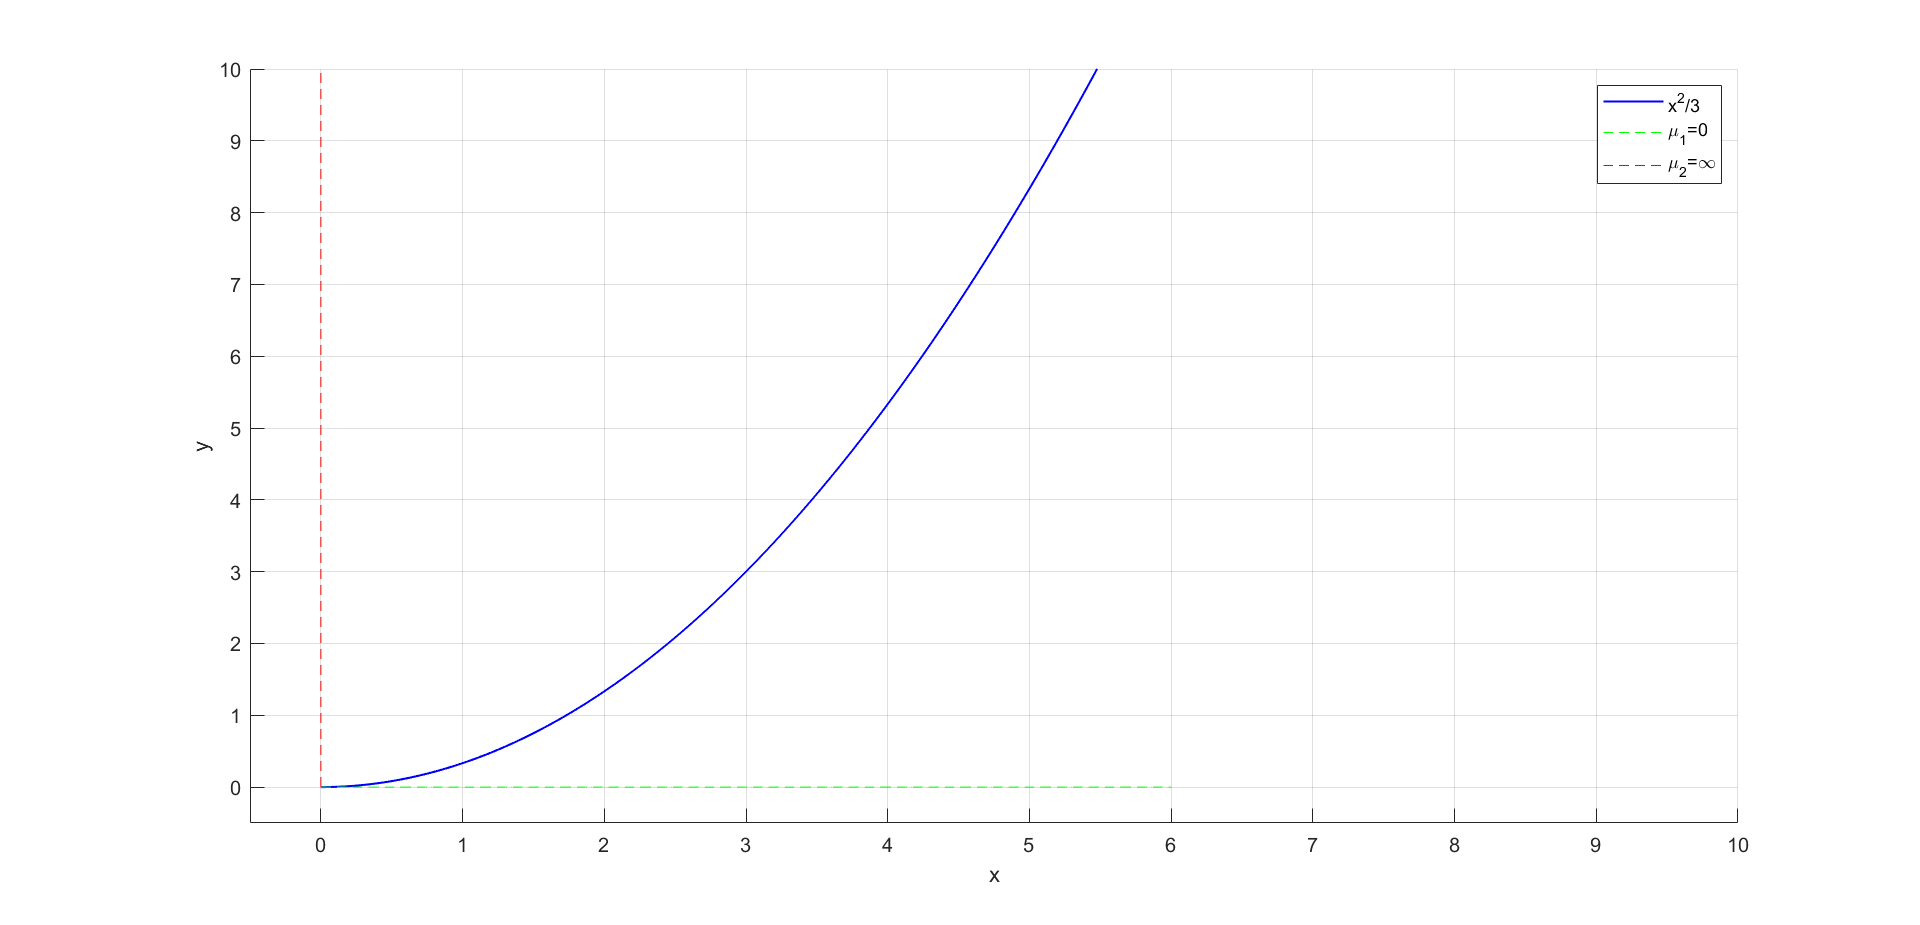
\includegraphics[width=0.7\textwidth]{sector_criterion_3}
    \caption{круговой критерий}
    \label{fig:sector_criterion_3}
\end{figure} \\
Из рисунка выше следует, что "секторное условие" выполнено.
\subsubsection*{Устойчивость матрицы $A$}
\[
det\{\lambda I - A\} = \lambda^2 -4\lambda + 2 \Rightarrow \lambda_1 = -2 + \sqrt{2}, \ \lambda_2 = -2 - \sqrt{2}
\]
Матрица $A$ устойчива.
\subsubsection*{"Частотное условие"}
Найдем передаточную функцию:
\[
W(\lambda) = c^T(A - \lambda I)^{-1}b = \frac{1}{\lambda^2 + 4\lambda+2}
\]
Возьмем $\lambda = i \omega$ и проверим выполнение неравенства:
\[
\mu_0^{-1} + Re[(1+i \omega \nu)W(i\omega)] > 0, \ \forall \omega \in [0, +\infty].
\]
Так как $\mu_0 = +\infty$, то $mu_0^{-1} = 0$. Получаем следующее неравенство:
\[
\begin{split}
Re[(1+i \omega \nu)W(i\omega)] = Re[(1+i \omega \nu)\frac{1}{-\omega^2 + i4\omega+2}] = Re[\frac{1+i \omega \nu}{-\omega^2 + i4\omega+2}] \\
= Re[\frac{2+2i \omega \nu - \omega^2 - i\omega^3\nu -i4\omega+4\omega^2\nu}{(2-\omega^2)^2 + 16\omega^2}] = \frac{4\omega^2\nu-\omega^2+2}{(2-\omega^2)^2 + 16\omega^2} = \frac{\omega^2(4\nu-1)+2}{(2-\omega^2)^2 + 16\omega^2}
\end{split}
\]
При $\nu \geq \frac{1}{4}$ числитель и знаменатель полученной дроби положительны при $\forall \omega$. \\
\ \\
Все условия теоремы выполнены, следовательно, система асимптотически устойчива.
\section*{Выводы}
В данной лабораторной работе исследовались нелинейные системы и способы оценки их устойчивости. В начале работы была проведена оценка устойчивости с помощью линеаризации и метода функций Ляпунова. Результаты расчетов были подтверждены графиками моделирования систем. В итоге, нелинейные системы можно успешно линеаризовывать около положения равновесия для анализа устойчивости в данной области.\\
Для доказательства экспоненциальной или асимптотической устойчивости использовались круговой критерий и критерий Попова соответственно. 
\end{document}